\subsection{Astrobiology System Design}
\label{sec:Astrobiology-Design}

The collection assembly was designed as a single mechanized enclosure as shown in the rendering in Figure \ref{fig:astrobiology-system} and the photograph shown in Figure \ref{fig:astrobiology-real}. The goal was to make this system fully autonomous with the use of a pressure sensor so that the arm would deploy once the balloon reached float altitude.  The rotating arm is raised out of the collection container and begins rotating once the payload reached float attitude. The raising of the rotating arms was done by a L-12 \SI{50}{\milli\meter} linear servo motor andthe rotation of the filter arm was provided by the rotational motor mounted onto the filter arm.  The lid on the top of the linear servo sealed the clean box during ascent and descent.  The Fluropore Membrane filters were mounted on the ends of the rotating arm.  The arms were set to spin at 80 RPM for the duration of float conditions.  In theory, the sampled volume is the cross-sectional area of each filter multiplied by the distance the payload traveled, resulting in a far greater sampled volume than the 0.03 liters per minute sampling of the pumps from the 2018 flight. When the payload began its descent from float conditions, the rotating arm would return to its home position and the linear actuator would retract the rotating mechanism back into the clean box.  The Fluropore filters on the rotation arm were compared with those mounted on the linear servo as shown in the figure below.  Background samples were taken using the same Fluropore membrane filters; these filters sampled the various places the payload was in, such as the UH lab room, the clean room used for sterilization, and the Fort Sumner launch site. This is done to take the possibility of contamination into consideration during the post-flight filter analysis.

\begin{figure}[h!]
	\begin{center}
	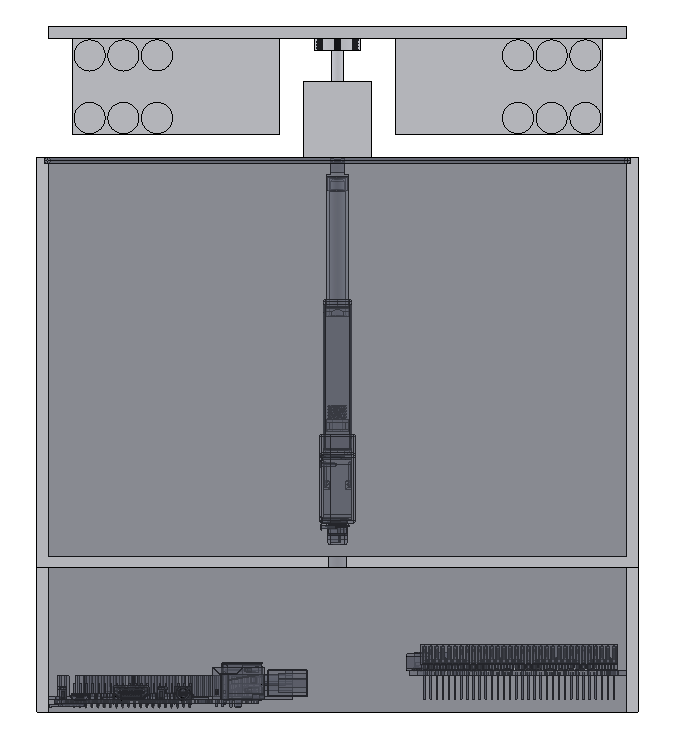
\includegraphics[width=0.65\textwidth]{figures/astrobio-electronics-deployed-transparent-sideview.png}
	\caption{Side view of the deployed astrobiology system mounted on top of the electronics box. The circles just beneath the lid mark the position and approximate size of the Fluropore filters.}
	\label{fig:astrobiology-system}
	\end{center}
\end{figure}

\begin{figure}[h!]
	\begin{center}
	\includegraphics[width=0.7\textwidth]{figures/astrobiology-container.jpg}
	\caption{Photograph of the astrobiology system prior to being sanitized and painted.}
	\label{fig:astrobiology-real}
	\end{center}
\end{figure}


